\documentclass[stu, 12pt, letterpaper, donotrepeattitle, floatsintext, natbib]{apa7}
\usepackage[utf8]{inputenc}
%\usepackage{fontspec} %paquete para usar la fuente Arial 12
\usepackage{comment}
\usepackage{marvosym}
\usepackage{graphicx}
\usepackage{float}
\usepackage[normalem]{ulem}
\usepackage[spanish]{babel} 
\usepackage{lastpage} %para le formato que quiere la profe QUITAR SI QUIERES OG APA7
\usepackage{ragged2e} %para le formato que quiere la profe QUITAR SI QUIERES OG APA7
\usepackage{indentfirst} %para le formato que quiere la profe QUITAR SI QUIERES OG APA7

\setcounter{secnumdepth}{0} %permite enumerar las secciones QUITAR SI QUIERES OG APA7

%comando para ajustar la fuente Arial en todo el documento
%\setmainfont{Arial} %COMPILAR DOC CON XeLateX DOS VECES

\DeclareCaptionLabelSeparator*{spaced}{\\[2ex]}
\captionsetup[table]{textfont=it,format=plain,justification=justified,
  singlelinecheck=false,labelsep=spaced,skip=1pt}

\selectlanguage{spanish}

\useunder{\uline}{\ul}{}
\newcommand{\myparagraph}[1]{\paragraph{#1}\mbox{}\\}

%\rfoot{Página \thepage \hspace{1pt} de \pageref{LastPage}}%QUITAR SI QUIERES OG APA7 
\rhead{} %QUITAR SI QUIERES OG APA7
\setcounter{secnumdepth}{3} %permite enumerar las secciones QUITAR SI QUIERES OG APA7
\setlength{\parindent}{1.27cm} %sangria forzada QUITAR SI QUIERES OG APA7

\renewcommand\labelitemi{$\bullet$}

\newcommand*\chem[1]{\ensuremath{\mathrm{#1}}}

\begin{document}
    %PORTADA
    \begin{titlepage}
        \begin{figure}[ht]
            \centering
            
\includegraphics[width=15cm]{logosITT.png}
        \end{figure}
        \centering
        {\Large Tecnológico Nacional de México\\Instituto Tecnológico de Tijuana\par}
        \vspace{1cm}
        {\Large SCD-1011SC6C Ingeniería de Software\par}
        \vspace{1cm}
        {\Large Unidad 2\par}
        \vspace{2cm}
        {\Large\bfseries Ejercicio 4\par}
        \vspace{2cm}
        {\large Dra. Martha Elena Pulido\par}
        \vfill
            {\large Abraham Jhared Flores Azcona, 19211640\par}
        \vfill
        {\large 10 de marzo de 2021}
    \end{titlepage}

% Índices
%\pagenumbering{arabic}
    % Contenido
%\renewcommand\contentsname{Contenido}
%\tableofcontents

% Cuerpo 
    %NOTA: PARA CITAR ESTILO "Merts (2003)" usar \cite{<nombre_cita_bib>}
    %                        "(Metz, 1978)" usar \citep{<nombre_cita_bib>}
\newpage
\section*{Diagrama UML de la actividad}
\begin{figure}[H]
    \caption{\emph{Diagrama de secuencia del escrito adjunto\\}}
    \centering
    \smallskip
    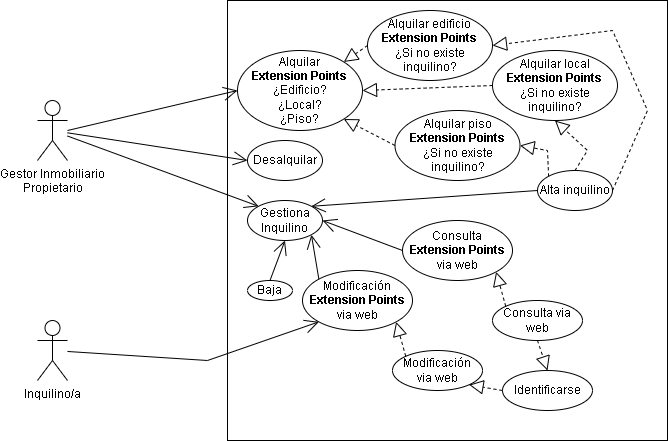
\includegraphics[width=14cm, height=16cm]{ejercicio4.png}
    \bigskip
    {\justifying\small\textit{\\Nota:} Autoría Propia (2022).}%citar al de medium del waterfall
\end{figure}
\end{document}